\subsection{Description/additional circuitry}
Car is using two torque encoders for accelerator pedal. Encoders are linear potentiometers. Sensors are powered and measured by ECU-P (electrical control unit - pedals). They output analog voltage signal equal to accelerator pedal position. Both output signals goes through \label{fig:ecup_analog_input} and low pass filters. Then they are fed to ADC (analog to digital converter) and analyzed by MCU (microcontroller unit) for validity and plausability. Information about position and errors is send though CAN.

\begin{table}[H]
	\centering
	\caption{Torque encoder data}
	\begin{tabularx}{\textwidth}{|X|X|}
		\hline
		Torque encoder manufacturer: & TE connectivity  \\[\TableSize]\hline
		Torque encoder type: & MLP-50  \\[\TableSize]\hline
		Torque encoder principle: & linear potentiometer  \\[\TableSize]\hline
		Total number of Torque Encoder Sensors: & 2  \\[\TableSize]\hline
		Supply voltage: & +5V  \\[\TableSize]\hline
		Maximum supply current: & 1mA  \\[\TableSize]\hline
		Operating temperature: & -30degC to -150degC  \\[\TableSize]\hline
		Used output: & DC voltage 0V to 5V\\[\TableSize]\hline
	\end{tabularx}%
	\label{tab:encoder-general}%
\end{table}%

\subsection{Torque Encoder Plausability Check}
Torque encoder implausability, short circuit and open circuit checks are done by MCU. Sensors are powered from +5V. Used travel of sensors does not contain end positions. Converted analog signal ranges are normalized according to calibration.
If any following sensor error is detected, motor controllers are shut down and message is send through CAN to other units.

\paragraph{Electrical check} 
Using only part of whole range of sensor excluding end positions allows detection of signal short to Ground or voltages higher or equal to sensor's power voltage.

Analog input circuitry of ECUP is shown in \ref{fig:ecup_analog_input}. In normal conditions, signal from sensor (RAW) goes through R2, then is clamped by D1 and continues through R1 and C1 to filters and other circuits of ECUP (AIN). TEST signal is held \textit{low} but due to high resistance of R3 has minimal impact on input signal.

When ADC measures 0V or value close to 0V, TEST signal logic level is switched \textit{high} to charge C1 through R3. After short while, logic level of TEST signal is read back. If \textit{high} logic level is read, sensor input is evaluated as \textit{open circuit}, otherwise it is \textit{short circuit} to GND. If measured value is close to power voltage of sensor or above measurable range, it is evaluated as \textit{short circuit} to power voltage or higher.

\paragraph{Implausability}
Position values difference is calculated and compared with maximal allowed error threshold (10\%).

\begin{figure}[H]
\begin{center}
	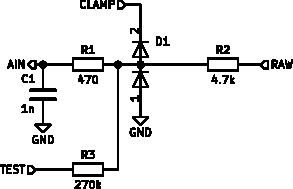
\includegraphics[width=0.5\textwidth]{./img/ECUP_AIN.pdf}
	\caption{ECU-P analog input circuit}
	\label{fig:ecup_analog_input}
\end{center}
\end{figure}



\subsection{Wiring}
\ref{fig:ecup_wiring} is diagram of sensor wiring.

\begin{figure}[H]
\begin{center}
	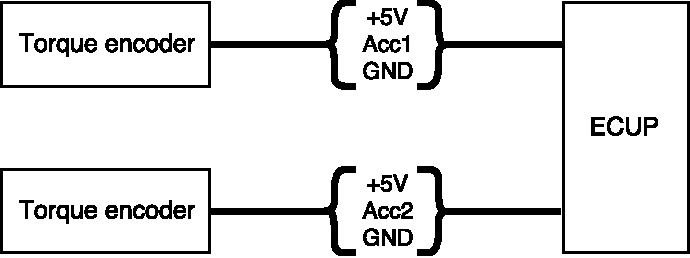
\includegraphics[width=0.5\textwidth]{./img/ECUP_wiring.pdf}
	\caption{ECU-P sensor wiring}
	\label{fig:ecup_wiring}
\end{center}
\end{figure}

\subsection{Position in car/mechanical fastening/mechanical connection}
In \ref{fig:torque_encoder_position} is shown position of two torque encoder sensors (piston shape objects).

\begin{figure}[H]
\begin{center}
	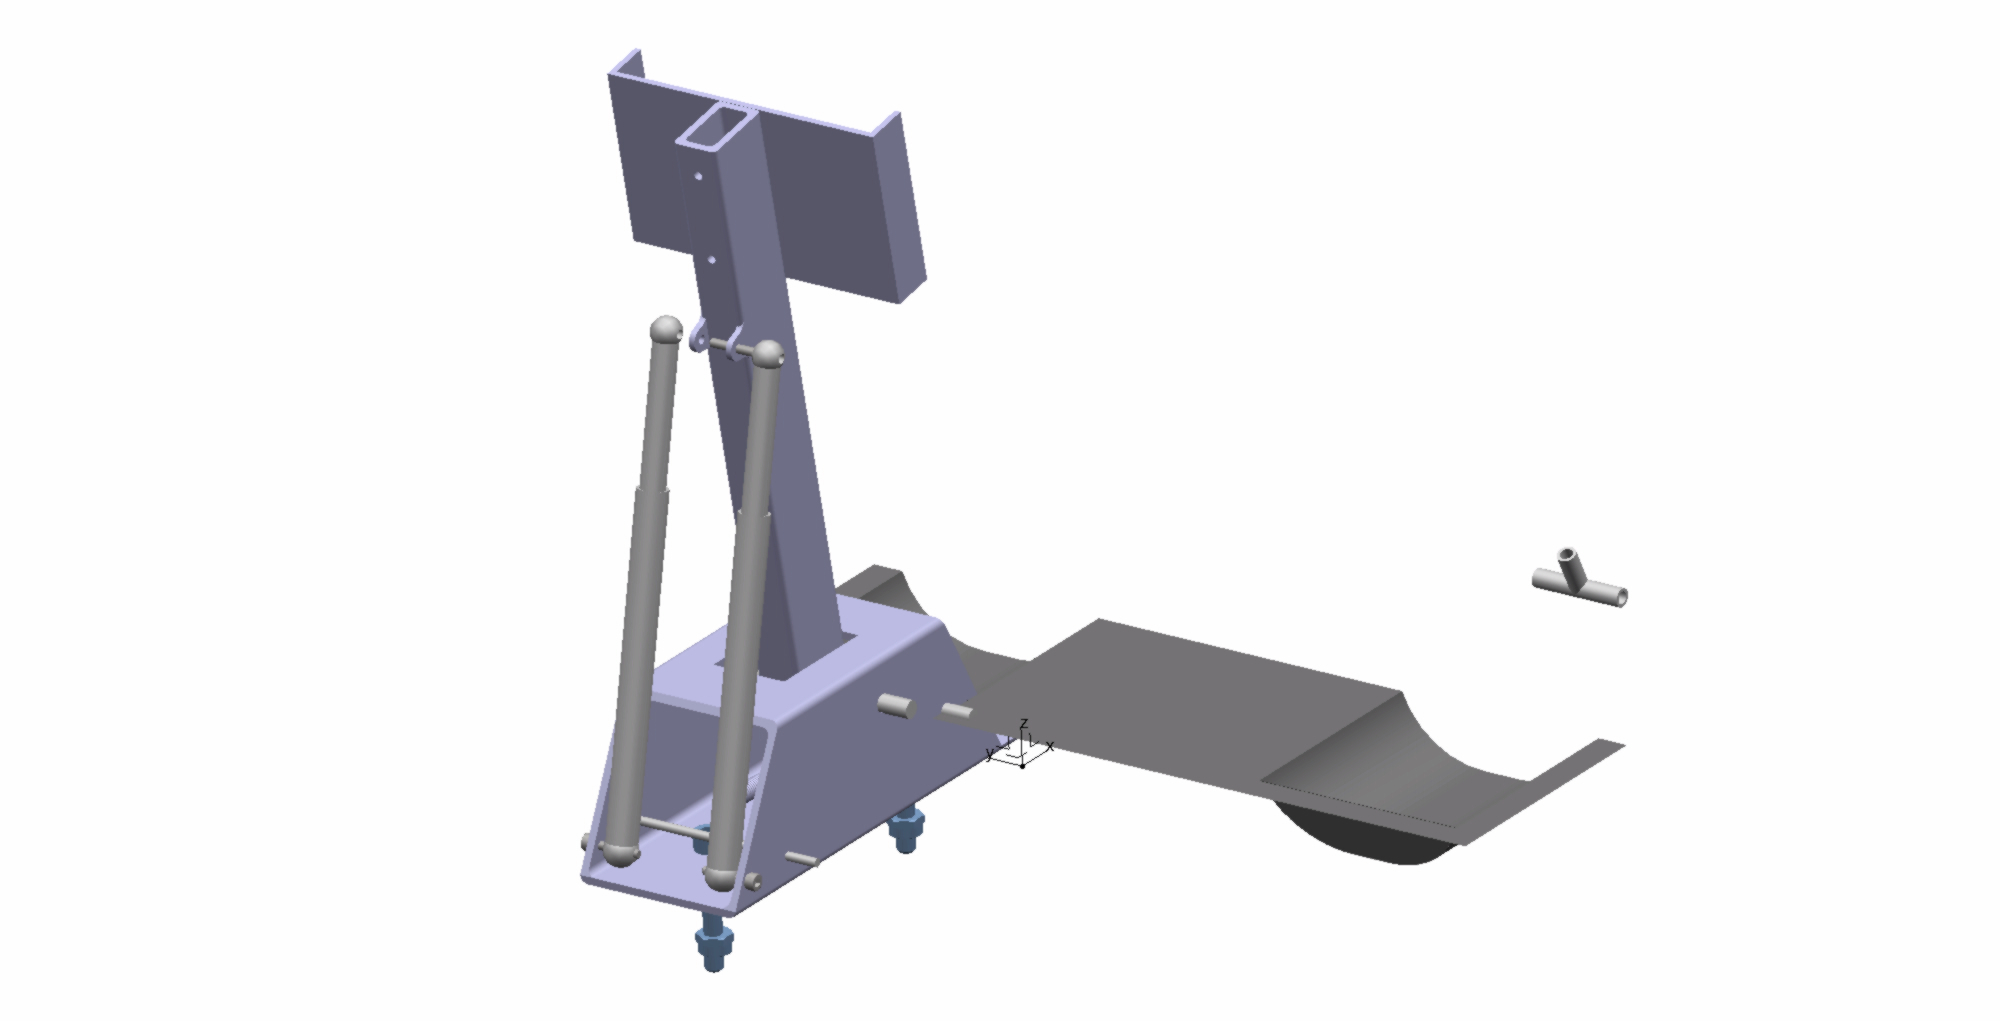
\includegraphics[width=0.8\textwidth]{./img/ACC-pedal-pos.jpg}
	\caption{Torque encoder position}
	\label{fig:torque_encoder_position}
\end{center}
\end{figure}



%\begin{figure}[H]
%\begin{center}
%	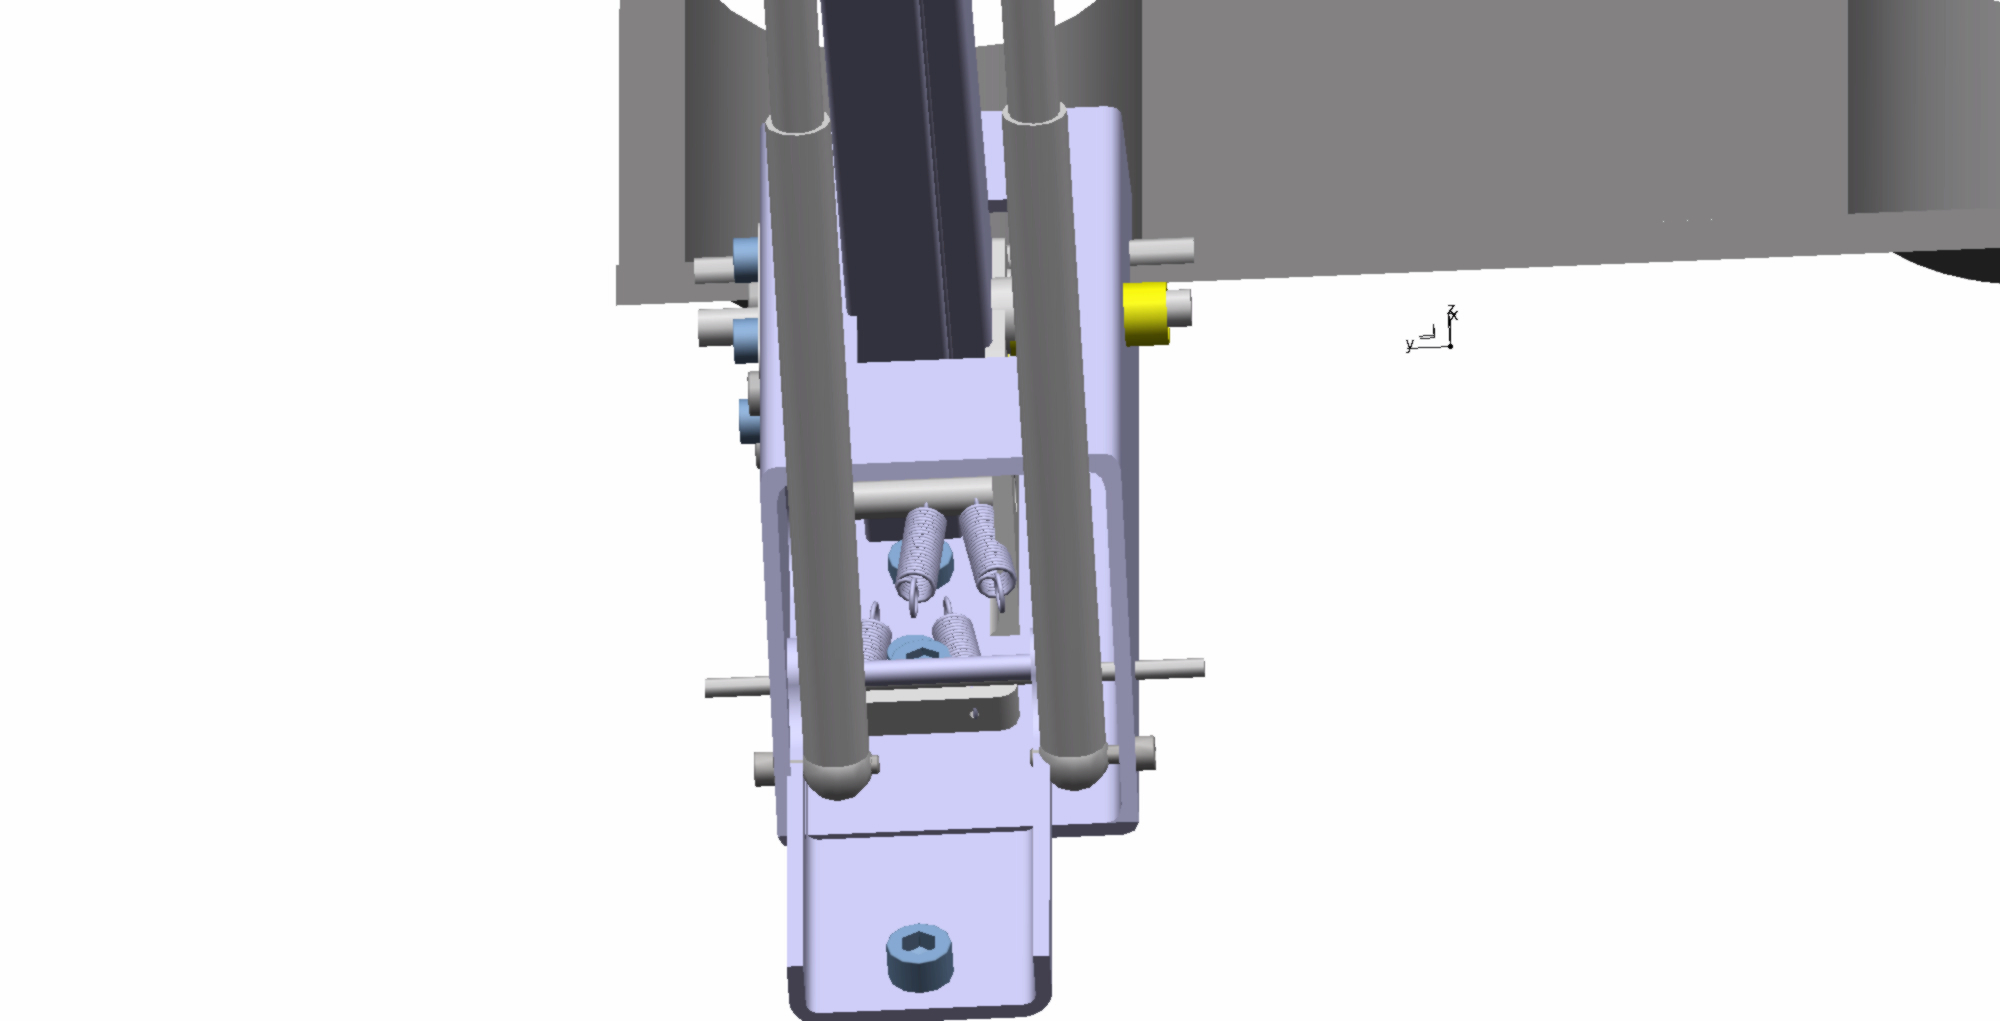
\includegraphics[width=0.8\textwidth]{./img/ACC-pedal-pos2.jpg}
%	\caption{Torque encoder position}
%	\label{fig:torque_encoder_position_alt}
%\end{center}
%\end{figure}


